\documentclass[1p]{elsarticle_modified}
%\bibliographystyle{elsarticle-num}

%\usepackage[colorlinks]{hyperref}
%\usepackage{abbrmath_seonhwa} %\Abb, \Ascr, \Acal ,\Abf, \Afrak
\usepackage{amsfonts}
\usepackage{amssymb}
\usepackage{amsmath}
\usepackage{amsthm}
\usepackage{scalefnt}
\usepackage{amsbsy}
\usepackage{kotex}
\usepackage{caption}
\usepackage{subfig}
\usepackage{color}
\usepackage{graphicx}
\usepackage{xcolor} %% white, black, red, green, blue, cyan, magenta, yellow
\usepackage{float}
\usepackage{setspace}
\usepackage{hyperref}

\usepackage{tikz}
\usetikzlibrary{arrows}

\usepackage{multirow}
\usepackage{array} % fixed length table
\usepackage{hhline}

%%%%%%%%%%%%%%%%%%%%%
\makeatletter
\renewcommand*\env@matrix[1][\arraystretch]{%
	\edef\arraystretch{#1}%
	\hskip -\arraycolsep
	\let\@ifnextchar\new@ifnextchar
	\array{*\c@MaxMatrixCols c}}
\makeatother %https://tex.stackexchange.com/questions/14071/how-can-i-increase-the-line-spacing-in-a-matrix
%%%%%%%%%%%%%%%

\usepackage[normalem]{ulem}

\newcommand{\msout}[1]{\ifmmode\text{\sout{\ensuremath{#1}}}\else\sout{#1}\fi}
%SOURCE: \msout is \stkout macro in https://tex.stackexchange.com/questions/20609/strikeout-in-math-mode

\newcommand{\cancel}[1]{
	\ifmmode
	{\color{red}\msout{#1}}
	\else
	{\color{red}\sout{#1}}
	\fi
}

\newcommand{\add}[1]{
	{\color{blue}\uwave{#1}}
}

\newcommand{\replace}[2]{
	\ifmmode
	{\color{red}\msout{#1}}{\color{blue}\uwave{#2}}
	\else
	{\color{red}\sout{#1}}{\color{blue}\uwave{#2}}
	\fi
}

\newcommand{\Sol}{\mathcal{S}} %segment
\newcommand{\D}{D} %diagram
\newcommand{\A}{\mathcal{A}} %arc


%%%%%%%%%%%%%%%%%%%%%%%%%%%%%5 test

\def\sl{\operatorname{\textup{SL}}(2,\Cbb)}
\def\psl{\operatorname{\textup{PSL}}(2,\Cbb)}
\def\quan{\mkern 1mu \triangleright \mkern 1mu}

\theoremstyle{definition}
\newtheorem{thm}{Theorem}[section]
\newtheorem{prop}[thm]{Proposition}
\newtheorem{lem}[thm]{Lemma}
\newtheorem{ques}[thm]{Question}
\newtheorem{cor}[thm]{Corollary}
\newtheorem{defn}[thm]{Definition}
\newtheorem{exam}[thm]{Example}
\newtheorem{rmk}[thm]{Remark}
\newtheorem{alg}[thm]{Algorithm}

\newcommand{\I}{\sqrt{-1}}
\begin{document}

%\begin{frontmatter}
%
%\title{Boundary parabolic representations of knots up to 8 crossings}
%
%%% Group authors per affiliation:
%\author{Yunhi Cho} 
%\address{Department of Mathematics, University of Seoul, Seoul, Korea}
%\ead{yhcho@uos.ac.kr}
%
%
%\author{Seonhwa Kim} %\fnref{s_kim}}
%\address{Center for Geometry and Physics, Institute for Basic Science, Pohang, 37673, Korea}
%\ead{ryeona17@ibs.re.kr}
%
%\author{Hyuk Kim}
%\address{Department of Mathematical Sciences, Seoul National University, Seoul 08826, Korea}
%\ead{hyukkim@snu.ac.kr}
%
%\author{Seokbeom Yoon}
%\address{Department of Mathematical Sciences, Seoul National University, Seoul, 08826,  Korea}
%\ead{sbyoon15@snu.ac.kr}
%
%\begin{abstract}
%We find all boundary parabolic representation of knots up to 8 crossings.
%
%\end{abstract}
%\begin{keyword}
%    \MSC[2010] 57M25 
%\end{keyword}
%
%\end{frontmatter}

%\linenumbers
%\tableofcontents
%
\newcommand\colored[1]{\textcolor{white}{\rule[-0.35ex]{0.8em}{1.4ex}}\kern-0.8em\color{red} #1}%
%\newcommand\colored[1]{\textcolor{white}{ #1}\kern-2.17ex	\textcolor{white}{ #1}\kern-1.81ex	\textcolor{white}{ #1}\kern-2.15ex\color{red}#1	}

{\Large $\underline{12n_{0139}~(K12n_{0139})}$}

\setlength{\tabcolsep}{10pt}
\renewcommand{\arraystretch}{1.6}
\vspace{1cm}\begin{tabular}{m{100pt}>{\centering\arraybackslash}m{274pt}}
\multirow{5}{120pt}{
	\centering
	\includegraphics[width=112pt]{../../../GIT/diagram.site/Diagrams/png/2228_12n_0139.png}\\
\ \ \ A knot diagram\footnotemark}&
\allowdisplaybreaks
\textbf{Linearized knot diagam} \\
\cline{2-2}
 &
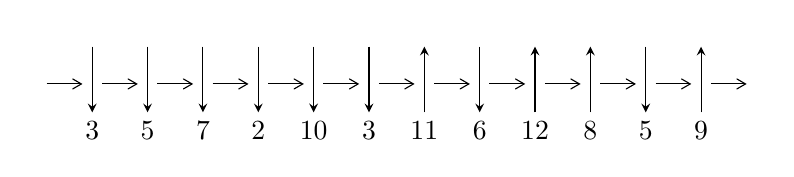
\begin{tikzpicture}[x=20pt, y=17pt]
	% nodes
	\node (C0) at (0, 0) {};
	\node (C1) at (1, 0) {};
	\node (C1U) at (1, +1) {};
	\node (C1D) at (1, -1) {3};

	\node (C2) at (2, 0) {};
	\node (C2U) at (2, +1) {};
	\node (C2D) at (2, -1) {5};

	\node (C3) at (3, 0) {};
	\node (C3U) at (3, +1) {};
	\node (C3D) at (3, -1) {7};

	\node (C4) at (4, 0) {};
	\node (C4U) at (4, +1) {};
	\node (C4D) at (4, -1) {2};

	\node (C5) at (5, 0) {};
	\node (C5U) at (5, +1) {};
	\node (C5D) at (5, -1) {10};

	\node (C6) at (6, 0) {};
	\node (C6U) at (6, +1) {};
	\node (C6D) at (6, -1) {3};

	\node (C7) at (7, 0) {};
	\node (C7U) at (7, +1) {};
	\node (C7D) at (7, -1) {11};

	\node (C8) at (8, 0) {};
	\node (C8U) at (8, +1) {};
	\node (C8D) at (8, -1) {6};

	\node (C9) at (9, 0) {};
	\node (C9U) at (9, +1) {};
	\node (C9D) at (9, -1) {12};

	\node (C10) at (10, 0) {};
	\node (C10U) at (10, +1) {};
	\node (C10D) at (10, -1) {8};

	\node (C11) at (11, 0) {};
	\node (C11U) at (11, +1) {};
	\node (C11D) at (11, -1) {5};

	\node (C12) at (12, 0) {};
	\node (C12U) at (12, +1) {};
	\node (C12D) at (12, -1) {9};
	\node (C13) at (13, 0) {};

	% arrows
	\draw[->,>={angle 60}]
	(C0) edge (C1) (C1) edge (C2) (C2) edge (C3) (C3) edge (C4) (C4) edge (C5) (C5) edge (C6) (C6) edge (C7) (C7) edge (C8) (C8) edge (C9) (C9) edge (C10) (C10) edge (C11) (C11) edge (C12) (C12) edge (C13) ;	\draw[->,>=stealth]
	(C1U) edge (C1D) (C2U) edge (C2D) (C3U) edge (C3D) (C4U) edge (C4D) (C5U) edge (C5D) (C6U) edge (C6D) (C7D) edge (C7U) (C8U) edge (C8D) (C9D) edge (C9U) (C10D) edge (C10U) (C11U) edge (C11D) (C12D) edge (C12U) ;
	\end{tikzpicture} \\
\hhline{~~} \\& 
\textbf{Solving Sequence} \\ \cline{2-2} 
 &
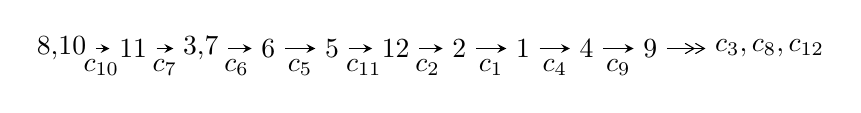
\begin{tikzpicture}[x=23pt, y=7pt]
	% node
	\node (A0) at (-1/8, 0) {8,10};
	\node (A1) at (1, 0) {11};
	\node (A2) at (33/16, 0) {3,7};
	\node (A3) at (25/8, 0) {6};
	\node (A4) at (33/8, 0) {5};
	\node (A5) at (41/8, 0) {12};
	\node (A6) at (49/8, 0) {2};
	\node (A7) at (57/8, 0) {1};
	\node (A8) at (65/8, 0) {4};
	\node (A9) at (73/8, 0) {9};
	\node (C1) at (1/2, -1) {$c_{10}$};
	\node (C2) at (3/2, -1) {$c_{7}$};
	\node (C3) at (21/8, -1) {$c_{6}$};
	\node (C4) at (29/8, -1) {$c_{5}$};
	\node (C5) at (37/8, -1) {$c_{11}$};
	\node (C6) at (45/8, -1) {$c_{2}$};
	\node (C7) at (53/8, -1) {$c_{1}$};
	\node (C8) at (61/8, -1) {$c_{4}$};
	\node (C9) at (69/8, -1) {$c_{9}$};
	\node (A10) at (11, 0) {$c_{3},c_{8},c_{12}$};

	% edge
	\draw[->,>=stealth]	
	(A0) edge (A1) (A1) edge (A2) (A2) edge (A3) (A3) edge (A4) (A4) edge (A5) (A5) edge (A6) (A6) edge (A7) (A7) edge (A8) (A8) edge (A9) ;
	\draw[->>,>={angle 60}]	
	(A9) edge (A10);
\end{tikzpicture} \\ 

\end{tabular} \\

\footnotetext{
The image of knot diagram is generated by the software ``\textbf{Draw programme}" developed by Andrew Bartholomew(\url{http://www.layer8.co.uk/maths/draw/index.htm\#Running-draw}), where we modified some parts for our purpose(\url{https://github.com/CATsTAILs/LinksPainter}).
}\phantom \\ \newline 
\centering \textbf{Ideals for irreducible components\footnotemark of $X_{\text{par}}$} 
 
\begin{align*}
I^u_{1}&=\langle 
1444693149 u^{23}-2063776507 u^{22}+\cdots+9741443072 b+4111548169,\\
\phantom{I^u_{1}}&\phantom{= \langle  }7418361699 u^{23}-17994094933 u^{22}+\cdots+19482886144 a+41117831143,\\
\phantom{I^u_{1}}&\phantom{= \langle  }u^{24}-2 u^{23}+\cdots+4 u+1\rangle \\
I^u_{2}&=\langle 
8.06000\times10^{26} u^{27}+4.92381\times10^{27} u^{26}+\cdots+6.21532\times10^{28} b+1.24378\times10^{29},\\
\phantom{I^u_{2}}&\phantom{= \langle  }-1.07145\times10^{29} u^{27}-9.17959\times10^{29} u^{26}+\cdots+6.02886\times10^{30} a-5.28882\times10^{31},\\
\phantom{I^u_{2}}&\phantom{= \langle  }u^{28}+6 u^{27}+\cdots+542 u+97\rangle \\
I^u_{3}&=\langle 
- u^3- u^2+2 b-2 u+1,\;u^3+3 u^2+4 a+2 u+1,\;u^4+u^2- u+1\rangle \\
I^u_{4}&=\langle 
- u^5- u^3- u^2+b- u-1,\;- u^4- u^2+a- u,\;u^6+u^5+2 u^4+2 u^3+2 u^2+2 u+1\rangle \\
I^u_{5}&=\langle 
-91 a^2 u-12 a^2+564 a u+337 b-570 a+147 u-188,\;a^3-7 a^2 u-5 a^2-4 a u- a+u-2,\;u^2+1\rangle \\
I^u_{6}&=\langle 
3 b+4 a+2,\;4 a^2-2 a-11,\;u-1\rangle \\
\\
\end{align*}
\raggedright * 6 irreducible components of $\dim_{\mathbb{C}}=0$, with total 70 representations.\\
\footnotetext{All coefficients of polynomials are rational numbers. But the coefficients are sometimes approximated in decimal forms when there is not enough margin.}
\newpage
\renewcommand{\arraystretch}{1}
\centering \section*{I. $I^u_{1}= \langle 1.44\times10^{9} u^{23}-2.06\times10^{9} u^{22}+\cdots+9.74\times10^{9} b+4.11\times10^{9},\;7.42\times10^{9} u^{23}-1.80\times10^{10} u^{22}+\cdots+1.95\times10^{10} a+4.11\times10^{10},\;u^{24}-2 u^{23}+\cdots+4 u+1 \rangle$}
\flushleft \textbf{(i) Arc colorings}\\
\begin{tabular}{m{7pt} m{180pt} m{7pt} m{180pt} }
\flushright $a_{8}=$&$\begin{pmatrix}0\\u\end{pmatrix}$ \\
\flushright $a_{10}=$&$\begin{pmatrix}1\\0\end{pmatrix}$ \\
\flushright $a_{11}=$&$\begin{pmatrix}1\\- u^2\end{pmatrix}$ \\
\flushright $a_{3}=$&$\begin{pmatrix}-0.380763 u^{23}+0.923585 u^{22}+\cdots+30.4809 u-2.11046\\-0.148304 u^{23}+0.211855 u^{22}+\cdots-1.81073 u-0.422068\end{pmatrix}$ \\
\flushright $a_{7}=$&$\begin{pmatrix}- u\\u^3+u\end{pmatrix}$ \\
\flushright $a_{6}=$&$\begin{pmatrix}0.0171864 u^{23}+0.103403 u^{22}+\cdots+13.2528 u-2.04858\\-0.192725 u^{23}+0.324632 u^{22}+\cdots+2.24962 u+0.0941446\end{pmatrix}$ \\
\flushright $a_{5}=$&$\begin{pmatrix}-0.175538 u^{23}+0.428035 u^{22}+\cdots+15.5024 u-1.95444\\-0.192725 u^{23}+0.324632 u^{22}+\cdots+2.24962 u+0.0941446\end{pmatrix}$ \\
\flushright $a_{12}=$&$\begin{pmatrix}-0.000122070 u^{23}+0.000366211 u^{22}+\cdots-3.00037 u+1.99988\\- u\end{pmatrix}$ \\
\flushright $a_{2}=$&$\begin{pmatrix}-0.343412 u^{23}+0.752066 u^{22}+\cdots+21.0006 u-1.27837\\-0.0361944 u^{23}-0.0124158 u^{22}+\cdots-3.46335 u-0.593642\end{pmatrix}$ \\
\flushright $a_{1}=$&$\begin{pmatrix}0.000244141 u^{23}-0.000732422 u^{22}+\cdots+4.00073 u-1.99976\\u^3+u\end{pmatrix}$ \\
\flushright $a_{4}=$&$\begin{pmatrix}-0.421620 u^{23}+0.978405 u^{22}+\cdots+30.4126 u-2.01569\\-0.0958427 u^{23}+0.0837108 u^{22}+\cdots-1.89080 u-0.543727\end{pmatrix}$ \\
\flushright $a_{9}=$&$\begin{pmatrix}-0.000122070 u^{23}+0.000366211 u^{22}+\cdots-2.00037 u+0.999878\\u^2\end{pmatrix}$\\&\end{tabular}
\flushleft \textbf{(ii) Obstruction class $= -1$}\\~\\
\flushleft \textbf{(iii) Cusp Shapes $= \frac{53447126663}{77931544576} u^{23}-\frac{86145029121}{77931544576} u^{22}+\cdots+\frac{1245910362157}{77931544576} u-\frac{821525338933}{77931544576}$}\\~\\
\newpage\renewcommand{\arraystretch}{1}
\flushleft \textbf{(iv) u-Polynomials at the component}\newline \\
\begin{tabular}{m{50pt}|m{274pt}}
Crossings & \hspace{64pt}u-Polynomials at each crossing \\
\hline $$\begin{aligned}c_{1}\end{aligned}$$&$\begin{aligned}
&u^{24}+26 u^{23}+\cdots-7007 u+256
\end{aligned}$\\
\hline $$\begin{aligned}c_{2},c_{4}\end{aligned}$$&$\begin{aligned}
&u^{24}-6 u^{23}+\cdots+u+16
\end{aligned}$\\
\hline $$\begin{aligned}c_{3},c_{6}\end{aligned}$$&$\begin{aligned}
&u^{24}+2 u^{23}+\cdots-96 u+256
\end{aligned}$\\
\hline $$\begin{aligned}c_{5}\end{aligned}$$&$\begin{aligned}
&u^{24}+6 u^{23}+\cdots+624 u+64
\end{aligned}$\\
\hline $$\begin{aligned}c_{7},c_{9},c_{10}\\c_{12}\end{aligned}$$&$\begin{aligned}
&u^{24}-2 u^{23}+\cdots+4 u+1
\end{aligned}$\\
\hline $$\begin{aligned}c_{8},c_{11}\end{aligned}$$&$\begin{aligned}
&4(4 u^{24}-10 u^{23}+\cdots+56 u+8)
\end{aligned}$\\
\hline
\end{tabular}\\~\\
\newpage\renewcommand{\arraystretch}{1}
\flushleft \textbf{(v) Riley Polynomials at the component}\newline \\
\begin{tabular}{m{50pt}|m{274pt}}
Crossings & \hspace{64pt}Riley Polynomials at each crossing \\
\hline $$\begin{aligned}c_{1}\end{aligned}$$&$\begin{aligned}
&y^{24}-50 y^{23}+\cdots-51129153 y+65536
\end{aligned}$\\
\hline $$\begin{aligned}c_{2},c_{4}\end{aligned}$$&$\begin{aligned}
&y^{24}-26 y^{23}+\cdots+7007 y+256
\end{aligned}$\\
\hline $$\begin{aligned}c_{3},c_{6}\end{aligned}$$&$\begin{aligned}
&y^{24}-18 y^{23}+\cdots-185344 y+65536
\end{aligned}$\\
\hline $$\begin{aligned}c_{5}\end{aligned}$$&$\begin{aligned}
&y^{24}+4 y^{23}+\cdots-69376 y+4096
\end{aligned}$\\
\hline $$\begin{aligned}c_{7},c_{9},c_{10}\\c_{12}\end{aligned}$$&$\begin{aligned}
&y^{24}+24 y^{23}+\cdots-110 y+1
\end{aligned}$\\
\hline $$\begin{aligned}c_{8},c_{11}\end{aligned}$$&$\begin{aligned}
&16(16 y^{24}-412 y^{23}+\cdots-64 y+64)
\end{aligned}$\\
\hline
\end{tabular}\\~\\
\newpage\flushleft \textbf{(vi) Complex Volumes and Cusp Shapes}
$$\begin{array}{c|c|c}  
\text{Solutions to }I^u_{1}& \I (\text{vol} + \sqrt{-1}CS) & \text{Cusp shape}\\
 \hline 
\begin{aligned}
u &= \phantom{-}1.08185\phantom{ +0.000000I} \\
a &= -2.32289\phantom{ +0.000000I} \\
b &= \phantom{-}4.49933\phantom{ +0.000000I}\end{aligned}
 & \phantom{-}0.548623\phantom{ +0.000000I} & -54.0530\phantom{ +0.000000I} \\ \hline\begin{aligned}
u &= \phantom{-}0.148994 + 0.783883 I \\
a &= -0.500058 - 0.355404 I \\
b &= -1.153660 - 0.222767 I\end{aligned}
 & \phantom{-}0.55362 + 3.41152 I & \phantom{-}0.86412 - 8.64734 I \\ \hline\begin{aligned}
u &= \phantom{-}0.148994 - 0.783883 I \\
a &= -0.500058 + 0.355404 I \\
b &= -1.153660 + 0.222767 I\end{aligned}
 & \phantom{-}0.55362 - 3.41152 I & \phantom{-}0.86412 + 8.64734 I \\ \hline\begin{aligned}
u &= \phantom{-}0.358870 + 1.163880 I \\
a &= \phantom{-}0.293497 + 0.216350 I \\
b &= \phantom{-}1.49300 - 0.50044 I\end{aligned}
 & -0.73599 - 1.30879 I & -8.68561 - 1.94237 I \\ \hline\begin{aligned}
u &= \phantom{-}0.358870 - 1.163880 I \\
a &= \phantom{-}0.293497 - 0.216350 I \\
b &= \phantom{-}1.49300 + 0.50044 I\end{aligned}
 & -0.73599 + 1.30879 I & -8.68561 + 1.94237 I \\ \hline\begin{aligned}
u &= -0.512568 + 1.179470 I \\
a &= \phantom{-}0.1243150 + 0.0579838 I \\
b &= \phantom{-}0.480003 + 0.040159 I\end{aligned}
 & -3.85211 - 7.19847 I & -3.15942 + 2.00992 I \\ \hline\begin{aligned}
u &= -0.512568 - 1.179470 I \\
a &= \phantom{-}0.1243150 - 0.0579838 I \\
b &= \phantom{-}0.480003 - 0.040159 I\end{aligned}
 & -3.85211 + 7.19847 I & -3.15942 - 2.00992 I \\ \hline\begin{aligned}
u &= \phantom{-}0.592376 + 0.366960 I \\
a &= -0.643909 + 0.233654 I \\
b &= \phantom{-}0.688451 + 0.658630 I\end{aligned}
 & \phantom{-}1.12915 + 1.02062 I & \phantom{-}4.27770 - 4.63248 I \\ \hline\begin{aligned}
u &= \phantom{-}0.592376 - 0.366960 I \\
a &= -0.643909 - 0.233654 I \\
b &= \phantom{-}0.688451 - 0.658630 I\end{aligned}
 & \phantom{-}1.12915 - 1.02062 I & \phantom{-}4.27770 + 4.63248 I \\ \hline\begin{aligned}
u &= -0.541907\phantom{ +0.000000I} \\
a &= \phantom{-}2.23521\phantom{ +0.000000I} \\
b &= -0.103995\phantom{ +0.000000I}\end{aligned}
 & -7.92944\phantom{ +0.000000I} & -16.4750\phantom{ +0.000000I}\\
 \hline 
 \end{array}$$\newpage$$\begin{array}{c|c|c}  
\text{Solutions to }I^u_{1}& \I (\text{vol} + \sqrt{-1}CS) & \text{Cusp shape}\\
 \hline 
\begin{aligned}
u &= -0.05535 + 1.55193 I \\
a &= -0.211228 + 1.127990 I \\
b &= -0.858668 + 0.189081 I\end{aligned}
 & -11.34610 - 0.73612 I & -10.72969 + 0.24360 I \\ \hline\begin{aligned}
u &= -0.05535 - 1.55193 I \\
a &= -0.211228 - 1.127990 I \\
b &= -0.858668 - 0.189081 I\end{aligned}
 & -11.34610 + 0.73612 I & -10.72969 - 0.24360 I \\ \hline\begin{aligned}
u &= \phantom{-}0.31630 + 1.54928 I \\
a &= \phantom{-}0.269994 - 1.060220 I \\
b &= -0.207846 - 0.286463 I\end{aligned}
 & -19.0579 + 6.6137 I & -10.93484 - 2.97293 I \\ \hline\begin{aligned}
u &= \phantom{-}0.31630 - 1.54928 I \\
a &= \phantom{-}0.269994 + 1.060220 I \\
b &= -0.207846 + 0.286463 I\end{aligned}
 & -19.0579 - 6.6137 I & -10.93484 + 2.97293 I \\ \hline\begin{aligned}
u &= -0.36560 + 1.55447 I \\
a &= \phantom{-}0.044155 - 1.334510 I \\
b &= \phantom{-}1.73078 - 0.39028 I\end{aligned}
 & -11.7462 - 9.1224 I & -9.90926 + 4.97595 I \\ \hline\begin{aligned}
u &= -0.36560 - 1.55447 I \\
a &= \phantom{-}0.044155 + 1.334510 I \\
b &= \phantom{-}1.73078 + 0.39028 I\end{aligned}
 & -11.7462 + 9.1224 I & -9.90926 - 4.97595 I \\ \hline\begin{aligned}
u &= -0.21985 + 1.60526 I \\
a &= -0.227686 - 0.153857 I \\
b &= -1.58817 - 0.13159 I\end{aligned}
 & -14.1758 - 4.9325 I & -11.00051 + 2.57629 I \\ \hline\begin{aligned}
u &= -0.21985 - 1.60526 I \\
a &= -0.227686 + 0.153857 I \\
b &= -1.58817 + 0.13159 I\end{aligned}
 & -14.1758 + 4.9325 I & -11.00051 - 2.57629 I \\ \hline\begin{aligned}
u &= \phantom{-}0.280085 + 0.207328 I \\
a &= \phantom{-}2.76775 + 0.68817 I \\
b &= -1.15139 - 0.84730 I\end{aligned}
 & -1.26399 + 0.69429 I & -5.88235 + 2.63444 I \\ \hline\begin{aligned}
u &= \phantom{-}0.280085 - 0.207328 I \\
a &= \phantom{-}2.76775 - 0.68817 I \\
b &= -1.15139 + 0.84730 I\end{aligned}
 & -1.26399 - 0.69429 I & -5.88235 - 2.63444 I\\
 \hline 
 \end{array}$$\newpage$$\begin{array}{c|c|c}  
\text{Solutions to }I^u_{1}& \I (\text{vol} + \sqrt{-1}CS) & \text{Cusp shape}\\
 \hline 
\begin{aligned}
u &= -0.62229 + 1.54349 I \\
a &= \phantom{-}0.33089 + 1.38912 I \\
b &= -2.20818 + 0.76804 I\end{aligned}
 & \phantom{-}19.7035 - 15.6516 I & -10.07185 + 6.64115 I \\ \hline\begin{aligned}
u &= -0.62229 - 1.54349 I \\
a &= \phantom{-}0.33089 - 1.38912 I \\
b &= -2.20818 - 0.76804 I\end{aligned}
 & \phantom{-}19.7035 + 15.6516 I & -10.07185 - 6.64115 I \\ \hline\begin{aligned}
u &= \phantom{-}1.71472\phantom{ +0.000000I} \\
a &= \phantom{-}1.29940\phantom{ +0.000000I} \\
b &= -4.00128\phantom{ +0.000000I}\end{aligned}
 & -8.86122\phantom{ +0.000000I} & -11.8540\phantom{ +0.000000I} \\ \hline\begin{aligned}
u &= -0.0966119\phantom{ +0.000000I} \\
a &= -5.95715\phantom{ +0.000000I} \\
b &= -0.342701\phantom{ +0.000000I}\end{aligned}
 & -0.870307\phantom{ +0.000000I} & -11.9670\phantom{ +0.000000I}\\
 \hline 
 \end{array}$$\newpage\newpage\renewcommand{\arraystretch}{1}
\centering \section*{II. $I^u_{2}= \langle 8.06\times10^{26} u^{27}+4.92\times10^{27} u^{26}+\cdots+6.22\times10^{28} b+1.24\times10^{29},\;-1.07\times10^{29} u^{27}-9.18\times10^{29} u^{26}+\cdots+6.03\times10^{30} a-5.29\times10^{31},\;u^{28}+6 u^{27}+\cdots+542 u+97 \rangle$}
\flushleft \textbf{(i) Arc colorings}\\
\begin{tabular}{m{7pt} m{180pt} m{7pt} m{180pt} }
\flushright $a_{8}=$&$\begin{pmatrix}0\\u\end{pmatrix}$ \\
\flushright $a_{10}=$&$\begin{pmatrix}1\\0\end{pmatrix}$ \\
\flushright $a_{11}=$&$\begin{pmatrix}1\\- u^2\end{pmatrix}$ \\
\flushright $a_{3}=$&$\begin{pmatrix}0.0177720 u^{27}+0.152261 u^{26}+\cdots+51.0589 u+8.77250\\-0.0129680 u^{27}-0.0792205 u^{26}+\cdots-10.1162 u-2.00116\end{pmatrix}$ \\
\flushright $a_{7}=$&$\begin{pmatrix}- u\\u^3+u\end{pmatrix}$ \\
\flushright $a_{6}=$&$\begin{pmatrix}0.0199647 u^{27}+0.149393 u^{26}+\cdots+34.2789 u+5.74653\\0.00250162 u^{27}-0.00246621 u^{26}+\cdots-4.44438 u-0.719728\end{pmatrix}$ \\
\flushright $a_{5}=$&$\begin{pmatrix}0.0224663 u^{27}+0.146927 u^{26}+\cdots+29.8346 u+5.02680\\0.00250162 u^{27}-0.00246621 u^{26}+\cdots-4.44438 u-0.719728\end{pmatrix}$ \\
\flushright $a_{12}=$&$\begin{pmatrix}0.153415 u^{27}+0.834186 u^{26}+\cdots-54.2701 u-12.9847\\-0.0420845 u^{27}-0.221294 u^{26}+\cdots-19.3117 u-4.11126\end{pmatrix}$ \\
\flushright $a_{2}=$&$\begin{pmatrix}0.0235732 u^{27}+0.167215 u^{26}+\cdots+33.8050 u+6.19640\\-0.00721990 u^{27}-0.0332133 u^{26}+\cdots-0.910549 u-0.565518\end{pmatrix}$ \\
\flushright $a_{1}=$&$\begin{pmatrix}0.0217420 u^{27}+0.116081 u^{26}+\cdots+1.22632 u+0.0581123\\u^3+u\end{pmatrix}$ \\
\flushright $a_{4}=$&$\begin{pmatrix}0.0203435 u^{27}+0.162178 u^{26}+\cdots+41.7784 u+6.36296\\0.000121206 u^{27}-0.0139096 u^{26}+\cdots-3.57361 u-0.126255\end{pmatrix}$ \\
\flushright $a_{9}=$&$\begin{pmatrix}-0.128091 u^{27}-0.908242 u^{26}+\cdots-122.754 u-18.4433\\0.0312135 u^{27}+0.163253 u^{26}+\cdots+18.6986 u+3.08220\end{pmatrix}$\\&\end{tabular}
\flushleft \textbf{(ii) Obstruction class $= -1$}\\~\\
\flushleft \textbf{(iii) Cusp Shapes $= -0.0158847 u^{27}-0.109997 u^{26}+\cdots-3.88785 u-3.25341$}\\~\\
\newpage\renewcommand{\arraystretch}{1}
\flushleft \textbf{(iv) u-Polynomials at the component}\newline \\
\begin{tabular}{m{50pt}|m{274pt}}
Crossings & \hspace{64pt}u-Polynomials at each crossing \\
\hline $$\begin{aligned}c_{1}\end{aligned}$$&$\begin{aligned}
&(u^{14}+20 u^{13}+\cdots+25 u+1)^{2}
\end{aligned}$\\
\hline $$\begin{aligned}c_{2},c_{4}\end{aligned}$$&$\begin{aligned}
&(u^{14}-4 u^{13}+\cdots- u-1)^{2}
\end{aligned}$\\
\hline $$\begin{aligned}c_{3},c_{6}\end{aligned}$$&$\begin{aligned}
&(u^{14}+u^{13}+\cdots+20 u+8)^{2}
\end{aligned}$\\
\hline $$\begin{aligned}c_{5}\end{aligned}$$&$\begin{aligned}
&(u^{14}-2 u^{13}+\cdots+4 u-1)^{2}
\end{aligned}$\\
\hline $$\begin{aligned}c_{7},c_{9},c_{10}\\c_{12}\end{aligned}$$&$\begin{aligned}
&u^{28}+6 u^{27}+\cdots+542 u+97
\end{aligned}$\\
\hline $$\begin{aligned}c_{8},c_{11}\end{aligned}$$&$\begin{aligned}
&u^{28}+2 u^{27}+\cdots-12530 u+4603
\end{aligned}$\\
\hline
\end{tabular}\\~\\
\newpage\renewcommand{\arraystretch}{1}
\flushleft \textbf{(v) Riley Polynomials at the component}\newline \\
\begin{tabular}{m{50pt}|m{274pt}}
Crossings & \hspace{64pt}Riley Polynomials at each crossing \\
\hline $$\begin{aligned}c_{1}\end{aligned}$$&$\begin{aligned}
&(y^{14}-48 y^{13}+\cdots-153 y+1)^{2}
\end{aligned}$\\
\hline $$\begin{aligned}c_{2},c_{4}\end{aligned}$$&$\begin{aligned}
&(y^{14}-20 y^{13}+\cdots-25 y+1)^{2}
\end{aligned}$\\
\hline $$\begin{aligned}c_{3},c_{6}\end{aligned}$$&$\begin{aligned}
&(y^{14}-21 y^{13}+\cdots-144 y+64)^{2}
\end{aligned}$\\
\hline $$\begin{aligned}c_{5}\end{aligned}$$&$\begin{aligned}
&(y^{14}-6 y^{13}+\cdots-8 y+1)^{2}
\end{aligned}$\\
\hline $$\begin{aligned}c_{7},c_{9},c_{10}\\c_{12}\end{aligned}$$&$\begin{aligned}
&y^{28}+22 y^{27}+\cdots+47288 y+9409
\end{aligned}$\\
\hline $$\begin{aligned}c_{8},c_{11}\end{aligned}$$&$\begin{aligned}
&y^{28}-22 y^{27}+\cdots+76721028 y+21187609
\end{aligned}$\\
\hline
\end{tabular}\\~\\
\newpage\flushleft \textbf{(vi) Complex Volumes and Cusp Shapes}
$$\begin{array}{c|c|c}  
\text{Solutions to }I^u_{2}& \I (\text{vol} + \sqrt{-1}CS) & \text{Cusp shape}\\
 \hline 
\begin{aligned}
u &= -0.121798 + 1.022010 I \\
a &= \phantom{-}2.24497 - 1.77780 I \\
b &= \phantom{-}0.448883\phantom{ +0.000000I}\end{aligned}
 & -4.07000\phantom{ +0.000000I} & -8.52950 + 0. I\phantom{ +0.000000I} \\ \hline\begin{aligned}
u &= -0.121798 - 1.022010 I \\
a &= \phantom{-}2.24497 + 1.77780 I \\
b &= \phantom{-}0.448883\phantom{ +0.000000I}\end{aligned}
 & -4.07000\phantom{ +0.000000I} & -8.52950 + 0. I\phantom{ +0.000000I} \\ \hline\begin{aligned}
u &= -0.730722 + 0.738022 I \\
a &= -1.55264 - 0.66750 I \\
b &= \phantom{-}1.94409 + 0.00042 I\end{aligned}
 & -6.39368 - 1.41191 I & -9.87318 + 3.81508 I \\ \hline\begin{aligned}
u &= -0.730722 - 0.738022 I \\
a &= -1.55264 + 0.66750 I \\
b &= \phantom{-}1.94409 - 0.00042 I\end{aligned}
 & -6.39368 + 1.41191 I & -9.87318 - 3.81508 I \\ \hline\begin{aligned}
u &= -0.961372 + 0.440888 I \\
a &= \phantom{-}1.47427 + 0.61493 I \\
b &= -1.88899 + 0.49296 I\end{aligned}
 & -5.27322 - 4.24963 I & -9.14655 + 5.18533 I \\ \hline\begin{aligned}
u &= -0.961372 - 0.440888 I \\
a &= \phantom{-}1.47427 - 0.61493 I \\
b &= -1.88899 - 0.49296 I\end{aligned}
 & -5.27322 + 4.24963 I & -9.14655 - 5.18533 I \\ \hline\begin{aligned}
u &= \phantom{-}0.778733 + 0.476869 I \\
a &= -0.560712 + 1.159950 I \\
b &= \phantom{-}0.091282 + 0.179107 I\end{aligned}
 & -12.49530 + 2.45847 I & -7.50081 - 0.42962 I \\ \hline\begin{aligned}
u &= \phantom{-}0.778733 - 0.476869 I \\
a &= -0.560712 - 1.159950 I \\
b &= \phantom{-}0.091282 - 0.179107 I\end{aligned}
 & -12.49530 - 2.45847 I & -7.50081 + 0.42962 I \\ \hline\begin{aligned}
u &= \phantom{-}0.396592 + 1.073210 I \\
a &= -0.365767 - 0.144675 I \\
b &= -0.597039 + 0.103194 I\end{aligned}
 & -0.91573 + 2.69540 I & \phantom{-}0.31936 - 2.88879 I \\ \hline\begin{aligned}
u &= \phantom{-}0.396592 - 1.073210 I \\
a &= -0.365767 + 0.144675 I \\
b &= -0.597039 - 0.103194 I\end{aligned}
 & -0.91573 - 2.69540 I & \phantom{-}0.31936 + 2.88879 I\\
 \hline 
 \end{array}$$\newpage$$\begin{array}{c|c|c}  
\text{Solutions to }I^u_{2}& \I (\text{vol} + \sqrt{-1}CS) & \text{Cusp shape}\\
 \hline 
\begin{aligned}
u &= -0.014446 + 1.158610 I \\
a &= \phantom{-}1.74504 + 1.57039 I \\
b &= \phantom{-}0.620567 - 0.112346 I\end{aligned}
 & -3.95002 - 0.09061 I & -6.51478 + 0.23122 I \\ \hline\begin{aligned}
u &= -0.014446 - 1.158610 I \\
a &= \phantom{-}1.74504 - 1.57039 I \\
b &= \phantom{-}0.620567 + 0.112346 I\end{aligned}
 & -3.95002 + 0.09061 I & -6.51478 - 0.23122 I \\ \hline\begin{aligned}
u &= -0.120439 + 0.677633 I \\
a &= -0.99346 - 2.55992 I \\
b &= \phantom{-}0.620567 + 0.112346 I\end{aligned}
 & -3.95002 + 0.09061 I & -6.51478 - 0.23122 I \\ \hline\begin{aligned}
u &= -0.120439 - 0.677633 I \\
a &= -0.99346 + 2.55992 I \\
b &= \phantom{-}0.620567 - 0.112346 I\end{aligned}
 & -3.95002 - 0.09061 I & -6.51478 + 0.23122 I \\ \hline\begin{aligned}
u &= -0.663607 + 0.149430 I \\
a &= \phantom{-}0.173852 + 0.543824 I \\
b &= -0.597039 + 0.103194 I\end{aligned}
 & -0.91573 + 2.69540 I & \phantom{-}0.31936 - 2.88879 I \\ \hline\begin{aligned}
u &= -0.663607 - 0.149430 I \\
a &= \phantom{-}0.173852 - 0.543824 I \\
b &= -0.597039 - 0.103194 I\end{aligned}
 & -0.91573 - 2.69540 I & \phantom{-}0.31936 + 2.88879 I \\ \hline\begin{aligned}
u &= -0.148951 + 1.396910 I \\
a &= -0.44526 - 1.43020 I \\
b &= \phantom{-}0.091282 - 0.179107 I\end{aligned}
 & -12.49530 - 2.45847 I & -7.50081 + 0.42962 I \\ \hline\begin{aligned}
u &= -0.148951 - 1.396910 I \\
a &= -0.44526 + 1.43020 I \\
b &= \phantom{-}0.091282 + 0.179107 I\end{aligned}
 & -12.49530 + 2.45847 I & -7.50081 - 0.42962 I \\ \hline\begin{aligned}
u &= -0.01413 + 1.43483 I \\
a &= \phantom{-}1.178910 - 0.382253 I \\
b &= \phantom{-}1.94409 - 0.00042 I\end{aligned}
 & -6.39368 + 1.41191 I & -9.87318 - 3.81508 I \\ \hline\begin{aligned}
u &= -0.01413 - 1.43483 I \\
a &= \phantom{-}1.178910 + 0.382253 I \\
b &= \phantom{-}1.94409 + 0.00042 I\end{aligned}
 & -6.39368 - 1.41191 I & -9.87318 + 3.81508 I\\
 \hline 
 \end{array}$$\newpage$$\begin{array}{c|c|c}  
\text{Solutions to }I^u_{2}& \I (\text{vol} + \sqrt{-1}CS) & \text{Cusp shape}\\
 \hline 
\begin{aligned}
u &= -1.47648 + 0.13393 I \\
a &= -1.255590 - 0.017191 I \\
b &= \phantom{-}2.70698 - 0.92539 I\end{aligned}
 & -14.4866 - 8.3929 I & -9.39875 + 4.58852 I \\ \hline\begin{aligned}
u &= -1.47648 - 0.13393 I \\
a &= -1.255590 + 0.017191 I \\
b &= \phantom{-}2.70698 + 0.92539 I\end{aligned}
 & -14.4866 + 8.3929 I & -9.39875 - 4.58852 I \\ \hline\begin{aligned}
u &= \phantom{-}0.23016 + 1.48936 I \\
a &= -0.53820 - 1.43603 I \\
b &= -1.88899 - 0.49296 I\end{aligned}
 & -5.27322 + 4.24963 I & -9.14655 - 5.18533 I \\ \hline\begin{aligned}
u &= \phantom{-}0.23016 - 1.48936 I \\
a &= -0.53820 + 1.43603 I \\
b &= -1.88899 + 0.49296 I\end{aligned}
 & -5.27322 - 4.24963 I & -9.14655 + 5.18533 I \\ \hline\begin{aligned}
u &= \phantom{-}0.64679 + 1.68867 I \\
a &= -0.104403 + 1.260500 I \\
b &= \phantom{-}2.70698 + 0.92539 I\end{aligned}
 & -14.4866 + 8.3929 I & -9.39875 - 4.58852 I \\ \hline\begin{aligned}
u &= \phantom{-}0.64679 - 1.68867 I \\
a &= -0.104403 - 1.260500 I \\
b &= \phantom{-}2.70698 - 0.92539 I\end{aligned}
 & -14.4866 - 8.3929 I & -9.39875 + 4.58852 I \\ \hline\begin{aligned}
u &= -0.80033 + 1.70926 I \\
a &= -0.068025 + 0.960101 I \\
b &= -3.20267\phantom{ +0.000000I}\end{aligned}
 & -19.1114\phantom{ +0.000000I} & -12.24106 + 0. I\phantom{ +0.000000I} \\ \hline\begin{aligned}
u &= -0.80033 - 1.70926 I \\
a &= -0.068025 - 0.960101 I \\
b &= -3.20267\phantom{ +0.000000I}\end{aligned}
 & -19.1114\phantom{ +0.000000I} & -12.24106 + 0. I\phantom{ +0.000000I}\\
 \hline 
 \end{array}$$\newpage\newpage\renewcommand{\arraystretch}{1}
\centering \section*{III. $I^u_{3}= \langle - u^3- u^2+2 b-2 u+1,\;u^3+3 u^2+4 a+2 u+1,\;u^4+u^2- u+1 \rangle$}
\flushleft \textbf{(i) Arc colorings}\\
\begin{tabular}{m{7pt} m{180pt} m{7pt} m{180pt} }
\flushright $a_{8}=$&$\begin{pmatrix}0\\u\end{pmatrix}$ \\
\flushright $a_{10}=$&$\begin{pmatrix}1\\0\end{pmatrix}$ \\
\flushright $a_{11}=$&$\begin{pmatrix}1\\- u^2\end{pmatrix}$ \\
\flushright $a_{3}=$&$\begin{pmatrix}-\frac{1}{4} u^3-\frac{3}{4} u^2-\frac{1}{2} u-\frac{1}{4}\\\frac{1}{2} u^3+\frac{1}{2} u^2+u-\frac{1}{2}\end{pmatrix}$ \\
\flushright $a_{7}=$&$\begin{pmatrix}- u\\u^3+u\end{pmatrix}$ \\
\flushright $a_{6}=$&$\begin{pmatrix}- u\\u^3+u\end{pmatrix}$ \\
\flushright $a_{5}=$&$\begin{pmatrix}u^3\\u^3+u\end{pmatrix}$ \\
\flushright $a_{12}=$&$\begin{pmatrix}- u^3+u^2- u+1\\- u\end{pmatrix}$ \\
\flushright $a_{2}=$&$\begin{pmatrix}-\frac{5}{4} u^3-\frac{3}{4} u^2-\frac{1}{2} u-\frac{1}{4}\\-\frac{1}{2} u^3+\frac{1}{2} u^2-\frac{1}{2}\end{pmatrix}$ \\
\flushright $a_{1}=$&$\begin{pmatrix}- u^3\\- u^3- u\end{pmatrix}$ \\
\flushright $a_{4}=$&$\begin{pmatrix}-\frac{1}{4} u^3-\frac{3}{4} u^2-\frac{1}{2} u-\frac{1}{4}\\\frac{1}{2} u^3+\frac{1}{2} u^2+u-\frac{1}{2}\end{pmatrix}$ \\
\flushright $a_{9}=$&$\begin{pmatrix}- u^3\\u^2\end{pmatrix}$\\&\end{tabular}
\flushleft \textbf{(ii) Obstruction class $= 1$}\\~\\
\flushleft \textbf{(iii) Cusp Shapes $= -\frac{79}{16} u^3-\frac{85}{16} u^2+\frac{21}{8} u-\frac{99}{16}$}\\~\\
\newpage\renewcommand{\arraystretch}{1}
\flushleft \textbf{(iv) u-Polynomials at the component}\newline \\
\begin{tabular}{m{50pt}|m{274pt}}
Crossings & \hspace{64pt}u-Polynomials at each crossing \\
\hline $$\begin{aligned}c_{1},c_{2}\end{aligned}$$&$\begin{aligned}
&(u-1)^4
\end{aligned}$\\
\hline $$\begin{aligned}c_{3},c_{6}\end{aligned}$$&$\begin{aligned}
&u^4
\end{aligned}$\\
\hline $$\begin{aligned}c_{4}\end{aligned}$$&$\begin{aligned}
&(u+1)^4
\end{aligned}$\\
\hline $$\begin{aligned}c_{5}\end{aligned}$$&$\begin{aligned}
&u^4+3 u^3+4 u^2+3 u+2
\end{aligned}$\\
\hline $$\begin{aligned}c_{7},c_{9}\end{aligned}$$&$\begin{aligned}
&u^4+u^2+u+1
\end{aligned}$\\
\hline $$\begin{aligned}c_{8},c_{11}\end{aligned}$$&$\begin{aligned}
&u^4+2 u^3+3 u^2+u+1
\end{aligned}$\\
\hline $$\begin{aligned}c_{10},c_{12}\end{aligned}$$&$\begin{aligned}
&u^4+u^2- u+1
\end{aligned}$\\
\hline
\end{tabular}\\~\\
\newpage\renewcommand{\arraystretch}{1}
\flushleft \textbf{(v) Riley Polynomials at the component}\newline \\
\begin{tabular}{m{50pt}|m{274pt}}
Crossings & \hspace{64pt}Riley Polynomials at each crossing \\
\hline $$\begin{aligned}c_{1},c_{2},c_{4}\end{aligned}$$&$\begin{aligned}
&(y-1)^4
\end{aligned}$\\
\hline $$\begin{aligned}c_{3},c_{6}\end{aligned}$$&$\begin{aligned}
&y^4
\end{aligned}$\\
\hline $$\begin{aligned}c_{5}\end{aligned}$$&$\begin{aligned}
&y^4- y^3+2 y^2+7 y+4
\end{aligned}$\\
\hline $$\begin{aligned}c_{7},c_{9},c_{10}\\c_{12}\end{aligned}$$&$\begin{aligned}
&y^4+2 y^3+3 y^2+y+1
\end{aligned}$\\
\hline $$\begin{aligned}c_{8},c_{11}\end{aligned}$$&$\begin{aligned}
&y^4+2 y^3+7 y^2+5 y+1
\end{aligned}$\\
\hline
\end{tabular}\\~\\
\newpage\flushleft \textbf{(vi) Complex Volumes and Cusp Shapes}
$$\begin{array}{c|c|c}  
\text{Solutions to }I^u_{3}& \I (\text{vol} + \sqrt{-1}CS) & \text{Cusp shape}\\
 \hline 
\begin{aligned}
u &= \phantom{-}0.547424 + 0.585652 I \\
a &= -0.391417 - 0.855136 I \\
b &= -0.173850 + 1.069070 I\end{aligned}
 & -0.66484 + 1.39709 I & -2.54919 - 3.47689 I \\ \hline\begin{aligned}
u &= \phantom{-}0.547424 - 0.585652 I \\
a &= -0.391417 + 0.855136 I \\
b &= -0.173850 - 1.069070 I\end{aligned}
 & -0.66484 - 1.39709 I & -2.54919 + 3.47689 I \\ \hline\begin{aligned}
u &= -0.547424 + 1.120870 I \\
a &= \phantom{-}0.266417 + 0.460085 I \\
b &= -0.576150 + 0.307015 I\end{aligned}
 & -4.26996 - 7.64338 I & -11.9196 + 11.4393 I \\ \hline\begin{aligned}
u &= -0.547424 - 1.120870 I \\
a &= \phantom{-}0.266417 - 0.460085 I \\
b &= -0.576150 - 0.307015 I\end{aligned}
 & -4.26996 + 7.64338 I & -11.9196 - 11.4393 I\\
 \hline 
 \end{array}$$\newpage\newpage\renewcommand{\arraystretch}{1}
\centering \section*{IV. $I^u_{4}= \langle - u^5- u^3- u^2+b- u-1,\;- u^4- u^2+a- u,\;u^6+u^5+2 u^4+2 u^3+2 u^2+2 u+1 \rangle$}
\flushleft \textbf{(i) Arc colorings}\\
\begin{tabular}{m{7pt} m{180pt} m{7pt} m{180pt} }
\flushright $a_{8}=$&$\begin{pmatrix}0\\u\end{pmatrix}$ \\
\flushright $a_{10}=$&$\begin{pmatrix}1\\0\end{pmatrix}$ \\
\flushright $a_{11}=$&$\begin{pmatrix}1\\- u^2\end{pmatrix}$ \\
\flushright $a_{3}=$&$\begin{pmatrix}u^4+u^2+u\\u^5+u^3+u^2+u+1\end{pmatrix}$ \\
\flushright $a_{7}=$&$\begin{pmatrix}- u\\u^3+u\end{pmatrix}$ \\
\flushright $a_{6}=$&$\begin{pmatrix}- u\\u^3+u\end{pmatrix}$ \\
\flushright $a_{5}=$&$\begin{pmatrix}u^3\\u^3+u\end{pmatrix}$ \\
\flushright $a_{12}=$&$\begin{pmatrix}u^4+u^2+u+1\\- u^5-2 u^3- u^2- u-1\end{pmatrix}$ \\
\flushright $a_{2}=$&$\begin{pmatrix}u^4- u^3+u^2+u\\u^5+u^2+1\end{pmatrix}$ \\
\flushright $a_{1}=$&$\begin{pmatrix}- u^3\\- u^3- u\end{pmatrix}$ \\
\flushright $a_{4}=$&$\begin{pmatrix}u^4+u^2+u\\u^5+u^3+u^2+u+1\end{pmatrix}$ \\
\flushright $a_{9}=$&$\begin{pmatrix}- u^3\\u^5+u^3+u\end{pmatrix}$\\&\end{tabular}
\flushleft \textbf{(ii) Obstruction class $= 1$}\\~\\
\flushleft \textbf{(iii) Cusp Shapes $= -2 u^5-5 u^3-2 u^2-5 u-12$}\\~\\
\newpage\renewcommand{\arraystretch}{1}
\flushleft \textbf{(iv) u-Polynomials at the component}\newline \\
\begin{tabular}{m{50pt}|m{274pt}}
Crossings & \hspace{64pt}u-Polynomials at each crossing \\
\hline $$\begin{aligned}c_{1},c_{2}\end{aligned}$$&$\begin{aligned}
&(u-1)^6
\end{aligned}$\\
\hline $$\begin{aligned}c_{3},c_{6}\end{aligned}$$&$\begin{aligned}
&u^6
\end{aligned}$\\
\hline $$\begin{aligned}c_{4}\end{aligned}$$&$\begin{aligned}
&(u+1)^6
\end{aligned}$\\
\hline $$\begin{aligned}c_{5}\end{aligned}$$&$\begin{aligned}
&(u^3- u^2+1)^2
\end{aligned}$\\
\hline $$\begin{aligned}c_{7},c_{9}\end{aligned}$$&$\begin{aligned}
&u^6- u^5+2 u^4-2 u^3+2 u^2-2 u+1
\end{aligned}$\\
\hline $$\begin{aligned}c_{8},c_{11}\end{aligned}$$&$\begin{aligned}
&u^6+3 u^5+4 u^4+2 u^3+1
\end{aligned}$\\
\hline $$\begin{aligned}c_{10},c_{12}\end{aligned}$$&$\begin{aligned}
&u^6+u^5+2 u^4+2 u^3+2 u^2+2 u+1
\end{aligned}$\\
\hline
\end{tabular}\\~\\
\newpage\renewcommand{\arraystretch}{1}
\flushleft \textbf{(v) Riley Polynomials at the component}\newline \\
\begin{tabular}{m{50pt}|m{274pt}}
Crossings & \hspace{64pt}Riley Polynomials at each crossing \\
\hline $$\begin{aligned}c_{1},c_{2},c_{4}\end{aligned}$$&$\begin{aligned}
&(y-1)^6
\end{aligned}$\\
\hline $$\begin{aligned}c_{3},c_{6}\end{aligned}$$&$\begin{aligned}
&y^6
\end{aligned}$\\
\hline $$\begin{aligned}c_{5}\end{aligned}$$&$\begin{aligned}
&(y^3- y^2+2 y-1)^2
\end{aligned}$\\
\hline $$\begin{aligned}c_{7},c_{9},c_{10}\\c_{12}\end{aligned}$$&$\begin{aligned}
&y^6+3 y^5+4 y^4+2 y^3+1
\end{aligned}$\\
\hline $$\begin{aligned}c_{8},c_{11}\end{aligned}$$&$\begin{aligned}
&y^6- y^5+4 y^4-2 y^3+8 y^2+1
\end{aligned}$\\
\hline
\end{tabular}\\~\\
\newpage\flushleft \textbf{(vi) Complex Volumes and Cusp Shapes}
$$\begin{array}{c|c|c}  
\text{Solutions to }I^u_{4}& \I (\text{vol} + \sqrt{-1}CS) & \text{Cusp shape}\\
 \hline 
\begin{aligned}
u &= \phantom{-}0.498832 + 1.001300 I \\
a &= -0.684695 + 0.494282 I \\
b &= \phantom{-}0.662359 + 0.562280 I\end{aligned}
 & -1.91067 + 2.82812 I & -8.69240 - 3.35914 I \\ \hline\begin{aligned}
u &= \phantom{-}0.498832 - 1.001300 I \\
a &= -0.684695 - 0.494282 I \\
b &= \phantom{-}0.662359 - 0.562280 I\end{aligned}
 & -1.91067 - 2.82812 I & -8.69240 + 3.35914 I \\ \hline\begin{aligned}
u &= -0.284920 + 1.115140 I \\
a &= -0.50000 + 1.95694 I \\
b &= -1.32472\phantom{ +0.000000I}\end{aligned}
 & -6.04826\phantom{ +0.000000I} & -9.61520 + 0. I\phantom{ +0.000000I} \\ \hline\begin{aligned}
u &= -0.284920 - 1.115140 I \\
a &= -0.50000 - 1.95694 I \\
b &= -1.32472\phantom{ +0.000000I}\end{aligned}
 & -6.04826\phantom{ +0.000000I} & -9.61520 + 0. I\phantom{ +0.000000I} \\ \hline\begin{aligned}
u &= -0.713912 + 0.305839 I \\
a &= -0.315305 - 0.494282 I \\
b &= \phantom{-}0.662359 + 0.562280 I\end{aligned}
 & -1.91067 + 2.82812 I & -8.69240 - 3.35914 I \\ \hline\begin{aligned}
u &= -0.713912 - 0.305839 I \\
a &= -0.315305 + 0.494282 I \\
b &= \phantom{-}0.662359 - 0.562280 I\end{aligned}
 & -1.91067 - 2.82812 I & -8.69240 + 3.35914 I\\
 \hline 
 \end{array}$$\newpage\newpage\renewcommand{\arraystretch}{1}
\centering \section*{V. $I^u_{5}= \langle -91 a^2 u+564 a u+\cdots-570 a-188,\;a^3-7 a^2 u-5 a^2-4 a u- a+u-2,\;u^2+1 \rangle$}
\flushleft \textbf{(i) Arc colorings}\\
\begin{tabular}{m{7pt} m{180pt} m{7pt} m{180pt} }
\flushright $a_{8}=$&$\begin{pmatrix}0\\u\end{pmatrix}$ \\
\flushright $a_{10}=$&$\begin{pmatrix}1\\0\end{pmatrix}$ \\
\flushright $a_{11}=$&$\begin{pmatrix}1\\1\end{pmatrix}$ \\
\flushright $a_{3}=$&$\begin{pmatrix}a\\0.270030 a^{2} u-1.67359 a u+\cdots+1.69139 a+0.557864\end{pmatrix}$ \\
\flushright $a_{7}=$&$\begin{pmatrix}- u\\0\end{pmatrix}$ \\
\flushright $a_{6}=$&$\begin{pmatrix}-0.0207715 a^{2} u-0.486647 a u+\cdots+0.0237389 a-0.504451\\0.121662 a^{2} u-0.721068 a u+\cdots+0.718101 a+0.240356\end{pmatrix}$ \\
\flushright $a_{5}=$&$\begin{pmatrix}0.100890 a^{2} u-1.20772 a u+\cdots+0.741840 a-0.264095\\0.121662 a^{2} u-0.721068 a u+\cdots+0.718101 a+0.240356\end{pmatrix}$ \\
\flushright $a_{12}=$&$\begin{pmatrix}0.136499 a^{2} u-0.516320 a u+\cdots+0.415430 a+0.172107\\u\end{pmatrix}$ \\
\flushright $a_{2}=$&$\begin{pmatrix}-0.0207715 a^{2} u-0.486647 a u+\cdots+0.0237389 a-0.504451\\0.121662 a^{2} u-0.721068 a u+\cdots+0.718101 a+0.240356\end{pmatrix}$ \\
\flushright $a_{1}=$&$\begin{pmatrix}u\\0\end{pmatrix}$ \\
\flushright $a_{4}=$&$\begin{pmatrix}0.270030 a^{2} u-1.67359 a u+\cdots+2.69139 a+0.557864\\0.270030 a^{2} u-1.67359 a u+\cdots+1.69139 a+0.557864\end{pmatrix}$ \\
\flushright $a_{9}=$&$\begin{pmatrix}-0.201780 a^{2} u+0.415430 a u+\cdots+0.516320 a+0.528190\\-1\end{pmatrix}$\\&\end{tabular}
\flushleft \textbf{(ii) Obstruction class $= 1$}\\~\\
\flushleft \textbf{(iii) Cusp Shapes $= \frac{56}{337} a^2 u-\frac{200}{337} a^2+\frac{1312}{337} a u+\frac{1284}{337} a+\frac{428}{337} u-\frac{2684}{337}$}\\~\\
\newpage\renewcommand{\arraystretch}{1}
\flushleft \textbf{(iv) u-Polynomials at the component}\newline \\
\begin{tabular}{m{50pt}|m{274pt}}
Crossings & \hspace{64pt}u-Polynomials at each crossing \\
\hline $$\begin{aligned}c_{1},c_{3}\end{aligned}$$&$\begin{aligned}
&(u^3- u^2+2 u-1)^2
\end{aligned}$\\
\hline $$\begin{aligned}c_{2}\end{aligned}$$&$\begin{aligned}
&(u^3+u^2-1)^2
\end{aligned}$\\
\hline $$\begin{aligned}c_{4}\end{aligned}$$&$\begin{aligned}
&(u^3- u^2+1)^2
\end{aligned}$\\
\hline $$\begin{aligned}c_{5}\end{aligned}$$&$\begin{aligned}
&u^6+5 u^4+10 u^2+1
\end{aligned}$\\
\hline $$\begin{aligned}c_{6}\end{aligned}$$&$\begin{aligned}
&(u^3+u^2+2 u+1)^2
\end{aligned}$\\
\hline $$\begin{aligned}c_{7},c_{9},c_{10}\\c_{12}\end{aligned}$$&$\begin{aligned}
&(u^2+1)^3
\end{aligned}$\\
\hline $$\begin{aligned}c_{8}\end{aligned}$$&$\begin{aligned}
&u^6-4 u^5+8 u^4+28 u^3+36 u^2+24 u+8
\end{aligned}$\\
\hline $$\begin{aligned}c_{11}\end{aligned}$$&$\begin{aligned}
&u^6+4 u^5+8 u^4-28 u^3+36 u^2-24 u+8
\end{aligned}$\\
\hline
\end{tabular}\\~\\
\newpage\renewcommand{\arraystretch}{1}
\flushleft \textbf{(v) Riley Polynomials at the component}\newline \\
\begin{tabular}{m{50pt}|m{274pt}}
Crossings & \hspace{64pt}Riley Polynomials at each crossing \\
\hline $$\begin{aligned}c_{1},c_{3},c_{6}\end{aligned}$$&$\begin{aligned}
&(y^3+3 y^2+2 y-1)^2
\end{aligned}$\\
\hline $$\begin{aligned}c_{2},c_{4}\end{aligned}$$&$\begin{aligned}
&(y^3- y^2+2 y-1)^2
\end{aligned}$\\
\hline $$\begin{aligned}c_{5}\end{aligned}$$&$\begin{aligned}
&(y^3+5 y^2+10 y+1)^2
\end{aligned}$\\
\hline $$\begin{aligned}c_{7},c_{9},c_{10}\\c_{12}\end{aligned}$$&$\begin{aligned}
&(y+1)^6
\end{aligned}$\\
\hline $$\begin{aligned}c_{8},c_{11}\end{aligned}$$&$\begin{aligned}
&y^6+360 y^4+80 y^2+64
\end{aligned}$\\
\hline
\end{tabular}\\~\\
\newpage\flushleft \textbf{(vi) Complex Volumes and Cusp Shapes}
$$\begin{array}{c|c|c}  
\text{Solutions to }I^u_{5}& \I (\text{vol} + \sqrt{-1}CS) & \text{Cusp shape}\\
 \hline 
\begin{aligned}
u &= \phantom{-0.000000 -}1.000000 I \\
a &= -0.567321 - 0.459293 I \\
b &= -1.307140 - 0.215080 I\end{aligned}
 & -0.26574 + 2.82812 I & -8.49024 - 2.97945 I \\ \hline\begin{aligned}
u &= \phantom{-0.000000 -}1.000000 I \\
a &= \phantom{-}0.163008 + 0.300102 I \\
b &= \phantom{-}1.307140 - 0.215080 I\end{aligned}
 & -0.26574 - 2.82812 I & -8.49024 + 2.97945 I \\ \hline\begin{aligned}
u &= \phantom{-0.000000 -}1.000000 I \\
a &= \phantom{-}5.40431 + 7.15919 I \\
b &= \phantom{-0.000000 } -0.569840 I\end{aligned}
 & -4.40332\phantom{ +0.000000I} & -15.0195 + 0. I\phantom{ +0.000000I} \\ \hline\begin{aligned}
u &= \phantom{-0.000000 } -1.000000 I \\
a &= -0.567321 + 0.459293 I \\
b &= -1.307140 + 0.215080 I\end{aligned}
 & -0.26574 - 2.82812 I & -8.49024 + 2.97945 I \\ \hline\begin{aligned}
u &= \phantom{-0.000000 } -1.000000 I \\
a &= \phantom{-}0.163008 - 0.300102 I \\
b &= \phantom{-}1.307140 + 0.215080 I\end{aligned}
 & -0.26574 + 2.82812 I & -8.49024 - 2.97945 I \\ \hline\begin{aligned}
u &= \phantom{-0.000000 } -1.000000 I \\
a &= \phantom{-}5.40431 - 7.15919 I \\
b &= \phantom{-0.000000 -}0.569840 I\end{aligned}
 & -4.40332\phantom{ +0.000000I} & -15.0195 + 0. I\phantom{ +0.000000I}\\
 \hline 
 \end{array}$$\newpage\newpage\renewcommand{\arraystretch}{1}
\centering \section*{VI. $I^u_{6}= \langle 3 b+4 a+2,\;4 a^2-2 a-11,\;u-1 \rangle$}
\flushleft \textbf{(i) Arc colorings}\\
\begin{tabular}{m{7pt} m{180pt} m{7pt} m{180pt} }
\flushright $a_{8}=$&$\begin{pmatrix}0\\1\end{pmatrix}$ \\
\flushright $a_{10}=$&$\begin{pmatrix}1\\0\end{pmatrix}$ \\
\flushright $a_{11}=$&$\begin{pmatrix}1\\-1\end{pmatrix}$ \\
\flushright $a_{3}=$&$\begin{pmatrix}a\\-\frac{4}{3} a-\frac{2}{3}\end{pmatrix}$ \\
\flushright $a_{7}=$&$\begin{pmatrix}-1\\2\end{pmatrix}$ \\
\flushright $a_{6}=$&$\begin{pmatrix}-\frac{1}{3} a+\frac{5}{6}\\0\end{pmatrix}$ \\
\flushright $a_{5}=$&$\begin{pmatrix}-\frac{1}{3} a+\frac{5}{6}\\0\end{pmatrix}$ \\
\flushright $a_{12}=$&$\begin{pmatrix}-\frac{1}{2} a+2\\-1\end{pmatrix}$ \\
\flushright $a_{2}=$&$\begin{pmatrix}\frac{1}{3} a+\frac{7}{6}\\-\frac{4}{3} a-\frac{2}{3}\end{pmatrix}$ \\
\flushright $a_{1}=$&$\begin{pmatrix}- a+3\\-2\end{pmatrix}$ \\
\flushright $a_{4}=$&$\begin{pmatrix}\frac{1}{3} a+\frac{2}{3}\\-2\end{pmatrix}$ \\
\flushright $a_{9}=$&$\begin{pmatrix}\frac{1}{2} a-1\\1\end{pmatrix}$\\&\end{tabular}
\flushleft \textbf{(ii) Obstruction class $= 1$}\\~\\
\flushleft \textbf{(iii) Cusp Shapes $= \frac{15}{2} a+7$}\\~\\
\newpage\renewcommand{\arraystretch}{1}
\flushleft \textbf{(iv) u-Polynomials at the component}\newline \\
\begin{tabular}{m{50pt}|m{274pt}}
Crossings & \hspace{64pt}u-Polynomials at each crossing \\
\hline $$\begin{aligned}c_{1}\end{aligned}$$&$\begin{aligned}
&u^2-3 u+1
\end{aligned}$\\
\hline $$\begin{aligned}c_{2},c_{3}\end{aligned}$$&$\begin{aligned}
&u^2+u-1
\end{aligned}$\\
\hline $$\begin{aligned}c_{4},c_{6}\end{aligned}$$&$\begin{aligned}
&u^2- u-1
\end{aligned}$\\
\hline $$\begin{aligned}c_{5}\end{aligned}$$&$\begin{aligned}
&u^2
\end{aligned}$\\
\hline $$\begin{aligned}c_{7},c_{9}\end{aligned}$$&$\begin{aligned}
&(u+1)^2
\end{aligned}$\\
\hline $$\begin{aligned}c_{8}\end{aligned}$$&$\begin{aligned}
&4(4 u^2+6 u+1)
\end{aligned}$\\
\hline $$\begin{aligned}c_{10},c_{12}\end{aligned}$$&$\begin{aligned}
&(u-1)^2
\end{aligned}$\\
\hline $$\begin{aligned}c_{11}\end{aligned}$$&$\begin{aligned}
&4(4 u^2-6 u+1)
\end{aligned}$\\
\hline
\end{tabular}\\~\\
\newpage\renewcommand{\arraystretch}{1}
\flushleft \textbf{(v) Riley Polynomials at the component}\newline \\
\begin{tabular}{m{50pt}|m{274pt}}
Crossings & \hspace{64pt}Riley Polynomials at each crossing \\
\hline $$\begin{aligned}c_{1}\end{aligned}$$&$\begin{aligned}
&y^2-7 y+1
\end{aligned}$\\
\hline $$\begin{aligned}c_{2},c_{3},c_{4}\\c_{6}\end{aligned}$$&$\begin{aligned}
&y^2-3 y+1
\end{aligned}$\\
\hline $$\begin{aligned}c_{5}\end{aligned}$$&$\begin{aligned}
&y^2
\end{aligned}$\\
\hline $$\begin{aligned}c_{7},c_{9},c_{10}\\c_{12}\end{aligned}$$&$\begin{aligned}
&(y-1)^2
\end{aligned}$\\
\hline $$\begin{aligned}c_{8},c_{11}\end{aligned}$$&$\begin{aligned}
&16(16 y^2-28 y+1)
\end{aligned}$\\
\hline
\end{tabular}\\~\\
\newpage\flushleft \textbf{(vi) Complex Volumes and Cusp Shapes}
$$\begin{array}{c|c|c}  
\text{Solutions to }I^u_{6}& \I (\text{vol} + \sqrt{-1}CS) & \text{Cusp shape}\\
 \hline 
\begin{aligned}
u &= \phantom{-}1.00000\phantom{ +0.000000I} \\
a &= -1.42705\phantom{ +0.000000I} \\
b &= \phantom{-}1.23607\phantom{ +0.000000I}\end{aligned}
 & -7.23771\phantom{ +0.000000I} & -3.70290\phantom{ +0.000000I} \\ \hline\begin{aligned}
u &= \phantom{-}1.00000\phantom{ +0.000000I} \\
a &= \phantom{-}1.92705\phantom{ +0.000000I} \\
b &= -3.23607\phantom{ +0.000000I}\end{aligned}
 & \phantom{-}0.657974\phantom{ +0.000000I} & \phantom{-}21.4530\phantom{ +0.000000I}\\
 \hline 
 \end{array}$$\newpage
\newpage\renewcommand{\arraystretch}{1}
\centering \section*{ VII. u-Polynomials}
\begin{tabular}{m{50pt}|m{274pt}}
Crossings & \hspace{64pt}u-Polynomials at each crossing \\
\hline $$\begin{aligned}c_{1}\end{aligned}$$&$\begin{aligned}
&(u-1)^{10}(u^2-3 u+1)(u^3- u^2+2 u-1)^2\\
&\cdot((u^{14}+20 u^{13}+\cdots+25 u+1)^{2})(u^{24}+26 u^{23}+\cdots-7007 u+256)
\end{aligned}$\\
\hline $$\begin{aligned}c_{2}\end{aligned}$$&$\begin{aligned}
&((u-1)^{10})(u^2+u-1)(u^3+u^2-1)^2(u^{14}-4 u^{13}+\cdots- u-1)^{2}\\
&\cdot(u^{24}-6 u^{23}+\cdots+u+16)
\end{aligned}$\\
\hline $$\begin{aligned}c_{3}\end{aligned}$$&$\begin{aligned}
&u^{10}(u^2+u-1)(u^3- u^2+2 u-1)^{2}(u^{14}+u^{13}+\cdots+20 u+8)^{2}\\
&\cdot(u^{24}+2 u^{23}+\cdots-96 u+256)
\end{aligned}$\\
\hline $$\begin{aligned}c_{4}\end{aligned}$$&$\begin{aligned}
&((u+1)^{10})(u^2- u-1)(u^3- u^2+1)^2(u^{14}-4 u^{13}+\cdots- u-1)^{2}\\
&\cdot(u^{24}-6 u^{23}+\cdots+u+16)
\end{aligned}$\\
\hline $$\begin{aligned}c_{5}\end{aligned}$$&$\begin{aligned}
&u^2(u^3- u^2+1)^2(u^4+3 u^3+4 u^2+3 u+2)(u^6+5 u^4+10 u^2+1)\\
&\cdot((u^{14}-2 u^{13}+\cdots+4 u-1)^{2})(u^{24}+6 u^{23}+\cdots+624 u+64)
\end{aligned}$\\
\hline $$\begin{aligned}c_{6}\end{aligned}$$&$\begin{aligned}
&u^{10}(u^2- u-1)(u^3+u^2+2 u+1)^{2}(u^{14}+u^{13}+\cdots+20 u+8)^{2}\\
&\cdot(u^{24}+2 u^{23}+\cdots-96 u+256)
\end{aligned}$\\
\hline $$\begin{aligned}c_{7},c_{9}\end{aligned}$$&$\begin{aligned}
&((u+1)^2)(u^2+1)^3(u^4+u^2+u+1)(u^6- u^5+\cdots-2 u+1)\\
&\cdot(u^{24}-2 u^{23}+\cdots+4 u+1)(u^{28}+6 u^{27}+\cdots+542 u+97)
\end{aligned}$\\
\hline $$\begin{aligned}c_{8}\end{aligned}$$&$\begin{aligned}
&16(4 u^2+6 u+1)(u^4+2 u^3+3 u^2+u+1)\\
&\cdot(u^6-4 u^5+\cdots+24 u+8)(u^6+3 u^5+4 u^4+2 u^3+1)\\
&\cdot(4 u^{24}-10 u^{23}+\cdots+56 u+8)(u^{28}+2 u^{27}+\cdots-12530 u+4603)
\end{aligned}$\\
\hline $$\begin{aligned}c_{10},c_{12}\end{aligned}$$&$\begin{aligned}
&((u-1)^2)(u^2+1)^3(u^4+u^2- u+1)(u^6+u^5+\cdots+2 u+1)\\
&\cdot(u^{24}-2 u^{23}+\cdots+4 u+1)(u^{28}+6 u^{27}+\cdots+542 u+97)
\end{aligned}$\\
\hline $$\begin{aligned}c_{11}\end{aligned}$$&$\begin{aligned}
&16(4 u^2-6 u+1)(u^4+2 u^3+\cdots+u+1)(u^{6}+3 u^{5}+\cdots+2 u^{3}+1)\\
&\cdot(u^6+4 u^5+\cdots-24 u+8)(4 u^{24}-10 u^{23}+\cdots+56 u+8)\\
&\cdot(u^{28}+2 u^{27}+\cdots-12530 u+4603)
\end{aligned}$\\
\hline
\end{tabular}\newpage\renewcommand{\arraystretch}{1}
\centering \section*{ VIII. Riley Polynomials}
\begin{tabular}{m{50pt}|m{274pt}}
Crossings & \hspace{64pt}Riley Polynomials at each crossing \\
\hline $$\begin{aligned}c_{1}\end{aligned}$$&$\begin{aligned}
&(y-1)^{10}(y^2-7 y+1)(y^3+3 y^2+2 y-1)^2\\
&\cdot(y^{14}-48 y^{13}+\cdots-153 y+1)^{2}\\
&\cdot(y^{24}-50 y^{23}+\cdots-51129153 y+65536)
\end{aligned}$\\
\hline $$\begin{aligned}c_{2},c_{4}\end{aligned}$$&$\begin{aligned}
&(y-1)^{10}(y^2-3 y+1)(y^3- y^2+2 y-1)^2\\
&\cdot((y^{14}-20 y^{13}+\cdots-25 y+1)^{2})(y^{24}-26 y^{23}+\cdots+7007 y+256)
\end{aligned}$\\
\hline $$\begin{aligned}c_{3},c_{6}\end{aligned}$$&$\begin{aligned}
&y^{10}(y^2-3 y+1)(y^{3}+3 y^{2}+2 y-1)^{2}(y^{14}-21 y^{13}+\cdots-144 y+64)^{2}\\
&\cdot(y^{24}-18 y^{23}+\cdots-185344 y+65536)
\end{aligned}$\\
\hline $$\begin{aligned}c_{5}\end{aligned}$$&$\begin{aligned}
&y^2(y^3- y^2+2 y-1)^2(y^3+5 y^2+10 y+1)^2(y^4- y^3+2 y^2+7 y+4)\\
&\cdot((y^{14}-6 y^{13}+\cdots-8 y+1)^{2})(y^{24}+4 y^{23}+\cdots-69376 y+4096)
\end{aligned}$\\
\hline $$\begin{aligned}c_{7},c_{9},c_{10}\\c_{12}\end{aligned}$$&$\begin{aligned}
&((y-1)^2)(y+1)^6(y^4+2 y^3+\cdots+y+1)(y^{6}+3 y^{5}+\cdots+2 y^{3}+1)\\
&\cdot(y^{24}+24 y^{23}+\cdots-110 y+1)(y^{28}+22 y^{27}+\cdots+47288 y+9409)
\end{aligned}$\\
\hline $$\begin{aligned}c_{8},c_{11}\end{aligned}$$&$\begin{aligned}
&256(16 y^2-28 y+1)(y^{4}+2 y^{3}+\cdots+5 y+1)(y^{6}+360 y^{4}+80 y^{2}+64)\\
&\cdot(y^6- y^5+4 y^4-2 y^3+8 y^2+1)(16 y^{24}-412 y^{23}+\cdots-64 y+64)\\
&\cdot(y^{28}-22 y^{27}+\cdots+76721028 y+21187609)
\end{aligned}$\\
\hline
\end{tabular}
\vskip 2pc
\end{document}